% AIAA Journal of Aircraft -- full research article -- DRAFT
%
% Build:  pdflatex paper && bibtex paper && pdflatex paper && pdflatex paper
% Class/style files live in style/ -- either compile with
%   TEXINPUTS=./style: BSTINPUTS=./style: pdflatex paper
% or copy aiaa-tc.cls and aiaa.bst next to this file.
%
% NOTE: style/aiaa-tc.cls and style/aiaa.bst were hand-extracted from the
% CTAN docstrip sources -- regenerate with `latex aiaa.ins` before a real
% submission (see README.md).
%
% STATUS: draft. Sections I-V are written against implemented, tested code.
% Section VI is written against the alpha/beta matrix exported by
% app/AttachmentSweepExport.cpp from the real geometry handoff; the figures
% come from figures/render-attachment-figures.py and the TABLES are
% generated by figures/render-coefficient-tables.py and \input-ed below, so
% no number in them is hand-typed. Rerun all three if the solver moves the
% numbers -- see README.md for the exact command sequence. Remaining before
% submission: author block details, acknowledgments, external validation,
% and regenerating the class files.

\documentclass[submit]{aiaa-tc}% journal mode: 12pt, double-spaced

\usepackage[utf8]{inputenc}
\usepackage{amsmath}
\usepackage{amssymb}
\usepackage{graphicx}
\usepackage{url}

\title{Aerodynamic Coefficients of a Coupled Wing--Body Configuration
       Across the Separation Boundary --- Part~I: Attachment Lines, the
       Separation March, and the Attached-Flow Envelope}

% Name diacritics confirmed. Still TODO before submission: the second
% author's department, the third author's faculty and email, and AIAA
% member grades for all three (same open item as the SciTech draft).
%
% Diacritics are written as LaTeX accent commands rather than literal
% UTF-8: aiaa-tc is an old class loaded without fontenc, and the Turkish
% letters break/dotted-I are outside the range inputenc alone handles
% reliably under pdflatex.
\author{
 Onur Tuncer%
  \thanks{Professor, Department of Aeronautical Engineering;
    onur.tuncer@itu.edu.tr. TODO: AIAA member grade.}\\
 {\normalsize\itshape
  Istanbul Technical University, Istanbul, T\"urkiye}
 \and
 \c{C}a\u{g}lar \"U\c{c}ler%
  \thanks{Associate Professor; caglar.ucler@ozyegin.edu.tr.
    TODO: department and AIAA member grade.}\\
 {\normalsize\itshape
  \"Ozye\u{g}in University, Istanbul, T\"urkiye}
 \and
 Ahmet G\"une\c{s}%
  \thanks{Associate Professor, Faculty of TODO; TODO: email and AIAA
    member grade.}\\
 {\normalsize\itshape
  Istanbul Technical University, Istanbul, T\"urkiye}
}

\newcommand{\eqnref}[1]{(\ref{#1})}
\newcommand{\Rbar}{\bar{R}}

\begin{document}

\maketitle

\begin{abstract}
Coupling a boundary-layer method to a potential-flow solver requires
knowing two things before the march can begin: where the flow attaches,
and what the edge-velocity distribution is measured from that point. This
paper presents a method for extracting both from a coupled wing--body
panel solve in which the lifting surfaces carry horseshoe vortices and the
fuselage carries constant-strength source panels in one blocked linear
system. The two halves of the airframe require different treatments, and
the difference is structural rather than incidental. A source-panelled
body is a real closed surface whose stagnation points exist in the
solution and are located by searching it; the skin-flow topology is
resolved in the panelling's own surface-index space, critical points are
found as common zeros of the contravariant velocity components, and they
are classified from a strain-rate tensor evaluated in a local orthonormal
frame. A vortex lattice, by contrast, is a zero-thickness camber sheet on
which the flow never stops, and no search of its field can produce an
attachment line. The lattice instead supplies the local induced flow to a
two-dimensional Hess--Smith solve of the section's reconstructed thick
contour, posed in the plane normal to the leading edge rather than
streamwise. That choice is shown to be load-bearing under sideslip: the
effective sweep moves in opposite directions on the two wings, so the
attachment line and its Reynolds number become asymmetric, and a
streamwise formulation returns a symmetric answer to an asymmetric
question. The method is verified against closed-form results --- exact
stagnation-point locations and strain rates on a sphere across the full
attitude range, exact surface velocity on a circular cylinder, and the
$\sqrt{r_{LE}}$ scaling of stagnation-point movement predicted by matched
asymptotics --- and yields, per spanwise station, the attachment-point
location, the Thwaites stagnation momentum thickness that starts a
chordwise march, and Poll's attachment-line Reynolds number.
\end{abstract}

\section*{Nomenclature}

\begin{tabbing}
  XXXXXXX \= \kill
  $\mathbf{a}_i, \mathbf{a}_j$ \> covariant surface basis vectors, m \\
  $b$ \> wing span, m \\
  $c$ \> streamwise chord, m \\
  $c_n$ \> chord in the leading-edge-normal plane, m \\
  $C_p$ \> pressure coefficient \\
  $C_L, C_{D_i}, C_Y$ \> lift, induced-drag and side-force coefficients \\
  $C_l, C_m, C_n$ \> rolling, pitching and yawing moment coefficients \\
  $h$ \> streamline divergence (spreading) metric \\
  $H$ \> boundary-layer shape factor \\
  $J$ \> surface strain-rate tensor, s$^{-1}$ \\
  $L$ \> body length, m \\
  $\hat{\mathbf{n}}$ \> unit outward surface normal \\
  $\Rbar$ \> attachment-line Reynolds number, $W_e \eta / \nu$ \\
  $r_{LE}$ \> leading-edge radius, m \\
  $s$ \> surface arc length, m \\
  $u, v$ \> contravariant surface velocity components, s$^{-1}$ \\
  $U_e$ \> boundary-layer edge velocity, m/s \\
  $\mathbf{V}_t$ \> surface-tangential velocity, m/s \\
  $W_e$ \> velocity component along the leading edge, m/s \\
  $\alpha$ \> angle of attack, deg \\
  $\alpha_n$ \> incidence in the leading-edge-normal plane, deg \\
  $\beta$ \> sideslip angle, deg \\
  $\Gamma$ \> circulation, m$^2$/s \\
  $\eta$ \> attachment-line length scale, $\sqrt{\nu/(dU_e/ds)}$, m \\
  $\theta$ \> momentum thickness, m \\
  $\lambda$ \> Thwaites' pressure-gradient parameter \\
  $\Lambda$ \> leading-edge sweep angle, deg \\
  $\Lambda_{\text{eff}}$ \> sweep relative to the local flow, deg \\
  $\nu$ \> kinematic viscosity, m$^2$/s \\
  $\sigma$ \> source-panel strength, m/s \\
  $\psi, \zeta$ \> section coordinates normalized by chord \\
\end{tabbing}

\section{Introduction}

Panel methods remain the workhorse of configuration-level aerodynamic
analysis because they resolve the inviscid field of a complete airframe in
seconds per operating point, which is what makes attitude sweeps,
stability-derivative tables and design optimization tractable. What they
do not resolve is the boundary layer, and the standard remedy --- coupling
an integral boundary-layer method to the inviscid
solution~\cite{cebeciCousteix2005,drela1989} --- has a prerequisite that
is easy to state and less easy to satisfy on a three-dimensional
configuration. Every integral method marches along an external streamline
from an attachment point. Before it can run, the attachment point must be
located and the edge velocity must be known as a function of arc length
measured from it.

On a two-dimensional airfoil this is routine: a panel method on the real
contour gives the surface velocity, whose sign change near the nose is the
stagnation point. On a three-dimensional airframe analyzed by a vortex
lattice it is not routine at all, for a reason that is worth making
explicit because it is frequently elided. A vortex lattice is not a model
of a surface. It is a model of a camber sheet of zero thickness, on which
the flow does not stop anywhere; the leading edge of such a sheet carries
a square-root velocity singularity rather than a stagnation point. Any
procedure that claims to locate a wing's attachment line by searching the
three-dimensional lattice field is therefore reporting a property of its
own discretization. The information required --- the leading-edge radius
and the surface curvature near it --- was discarded when the section was
reduced to its mean line.

A source-panelled body is in the opposite position. It is a genuine closed
surface carrying a genuine velocity field, and its stagnation points exist
in the solution as zeros of the surface-tangential velocity. They can be
found rather than modeled, together with the whole skin-flow topology:
attachment and separation nodes, saddles whose separatrices divide the
surface, and foci marking vortical
liftoff~\cite{lighthill1963,tobakPeake1982}.

This paper presents a treatment that respects that asymmetry rather than
papering over it, implemented in an open-source coupled wing--body--
propeller solver~\cite{aeolion2026}. Section~\ref{sec:formulation}
summarizes the coupled vortex/source system and the velocity-field
abstraction both halves are built on. Section~\ref{sec:body} develops the
body skin-flow analysis. Section~\ref{sec:wing} develops the wing
attachment line, posed in leading-edge-normal coordinates, and argues that
this choice is forced --- not merely preferable --- once sideslip is
admitted. Section~\ref{sec:verification} verifies both against closed-form
results. This part carries the aerodynamics \emph{up to} the separation
boundary: the coefficient and derivative tables it produces are
truncated where the march says separation takes over. What lies beyond
that boundary --- the post-separation coefficients toward the
flat-plate limit --- is the subject of Part~II of this series.

The motivating application is an attitude sweep. Angle of attack and
sideslip are the two parameters a stability and control analysis varies
most, and they move the attachment line in qualitatively different ways:
$\alpha$ walks it chordwise, symmetrically; $\beta$ moves it
\emph{asymmetrically} on a swept wing and rotates the body's stagnation
point about the fuselage axis. The second effect has consequences for
transition that a symmetric treatment cannot represent.

\section{Formulation}
\label{sec:formulation}

\subsection{The coupled wing--body system}

Lifting surfaces are discretized into horseshoe-vortex panels with bound
segments on the local quarter-chord line and flow tangency enforced at the
three-quarter-chord point. The fuselage is discretized into
constant-strength quadrilateral source panels: a source distribution
enforces zero through-flow on a closed non-lifting volume without
introducing bound circulation or a shed wake, which paneling a fuselage
with horseshoes would incorrectly do. Sources produce no net force on a
closed body, as d'Alembert requires, but they do produce the surface
pressure distribution and hence the Munk moment~\cite{munk1924}, and the
upwash the wing sees.

The two are not solved separately and then superposed. There is one
system, in which every unknown is a singularity strength and every
equation is flow tangency at a control point:
%
\begin{equation}
  \label{eq:blocked}
  \begin{bmatrix} A_{vv} & A_{vs} \\ A_{sv} & A_{ss} \end{bmatrix}
  \begin{Bmatrix} \Gamma \\ \sigma \end{Bmatrix}
  =
  \begin{Bmatrix} w_v - \mathbf{V}_{\text{kin}}\cdot\hat{\mathbf{n}}_v \\
                  w_s - \mathbf{V}_{\text{kin}}\cdot\hat{\mathbf{n}}_s \end{Bmatrix}
\end{equation}
%
where $A_{xy}$ is the normal velocity induced at an $x$ control point by
unit strength on a $y$ element and $w$ is the prescribed normal velocity,
zero on any solid surface. The blocking is emergent rather than
constructed: unknowns are indexed vortices first, then sources, so the
four blocks are regions of one matrix filled by one loop. A wing-only case
is the same system with the source rows and columns absent.

In-plane source influence follows the classical Hess--Smith flat-panel
result~\cite{hessSmith1962,katzPlotkin2001}. The normal component is taken
as the signed solid angle the panel subtends at the field point, evaluated
per triangle by the van Oosterom--Strackee
formula~\cite{vanOosteromStrackee1983} rather than by the textbook
per-edge arctangent form, which is singular for any edge parallel to a
local axis --- a case that arises constantly on a body of revolution.

\subsection{The velocity field as a first-class object}
\label{sec:flowfield}

Both analyses that follow must evaluate velocity \emph{after} the solve,
at points that are not control points. This is a modest but consequential
change in how a panel solver is structured: the field is made an explicit
object carrying the converged $\Gamma$ and $\sigma$, and the force
integration is rewritten to go through it, so that no second definition of
``the velocity here'' exists to drift from the first.

Three evaluations are distinguished, and neither of the special cases is
an approximation of the general one. The plain field applies at an
arbitrary point. At a panel's own bound-vortex midpoint that segment is
singular and is excluded, because Kutta--Joukowski requires the flow the
segment sits \emph{in}, not the flow it creates. At a source panel's own
control point --- which lies exactly on its own sheet, where the induced
velocity is indeterminate --- the analytic $+\tfrac12$ sheet jump is
substituted, the in-plane part canceling by symmetry.

\section{Body skin-flow topology}
\label{sec:body}

\subsection{Surface coordinates}

The analysis is carried out in the paneling's own $(i,j)$ index space ---
axial station and azimuthal sector --- rather than in a body-fixed
$(x,\phi)$. Recovering an azimuth as $\arctan(z/y)$ presumes the surface
is swept about a particular axis through the origin, which is true of a
fuselage, false of an offset duct or nacelle, and \emph{silently} false:
the failure mode is a streamline that curves incorrectly, not an error.
Each panel therefore states its own surface indices, and a patch that does
not state a complete topology is declined rather than reconstructed.

Index space requires a metric, carried on the grid:
%
\begin{equation}
  \mathbf{a}_i = \frac{\partial \mathbf{P}}{\partial i}, \quad
  \mathbf{a}_j = \frac{\partial \mathbf{P}}{\partial j}, \quad
  \mathbf{V}_t = u\,\mathbf{a}_i + v\,\mathbf{a}_j, \quad
  \sqrt{g} = |\mathbf{a}_i \times \mathbf{a}_j| .
\end{equation}
%
The contravariant components $(u,v)$ are obtained once per node from the
$2\times2$ Gram system and stored. Because the Gram matrix is positive
definite, they vanish exactly where $\mathbf{V}_t$ does, which reduces the
search for stagnation points to the search for a common zero of two
bilinear interpolants: cells across whose corners both components change
sign are candidates, and a two-dimensional Newton iteration locates the
zero within one.

\subsection{Classification}

A critical point is classified from the Jacobian of the surface flow. The
eigenvalues are coordinate-independent: where the velocity vanishes, a
change of surface coordinate maps $J \mapsto M J M^{-1}$, the term
involving the derivative of $M$ being multiplied by a velocity that is
zero. Node, saddle and focus, and the attachment/separation distinction,
are therefore properties of the flow and not of the chart. Surface
streamlines run along $\mathbf{V}_t$, so flow \emph{arrives} and spreads
at an attachment point and its eigenvalues have positive real parts.

Two numerical points determine whether this is usable in practice.

First, the Jacobian is \emph{not} differenced from $(u,v)$. Those are not
smooth fields even where the flow is: on a body of revolution the
azimuthal basis vector shrinks with local radius, so $v$ carries a $1/r$
factor that varies by tens of percent across a single cell near a nose.
Interpolating it is harmless --- it is exact at the nodes, which is all a
streamline integrator requires --- but differencing it folds the chart's
own distortion into the result. Measured on a sphere, whose stagnation
node is exactly isotropic, this produces a spurious 2:1 eigenvalue split.
The strain rate is instead obtained by differencing the tangential
velocity vector in a local orthonormal frame, which makes $J$ a physical
strain rate in s$^{-1}$.

Second, a focus is declared only when the point genuinely spirals. An
isotropic node lies exactly on the node/focus boundary, where the
discriminant vanishes; a bare sign test on the discriminant reports a
sphere's forward stagnation point as a spiral under any perturbation. The
implementation requires $|\mathrm{Im}\,\lambda|$ to reach a quarter of
$|\mathrm{Re}\,\lambda|$, reserving the classification for the vortical
separation it is meant to name.

\subsection{Streamlines and the spreading metric}

Surface streamlines are integrated with fourth-order Runge--Kutta in index
space, so that a step is a fixed fraction of a \emph{cell} rather than of
a length --- the natural step for a mesh whose cells vary in size along
the body. Near a critical point the field is $\dot{\xi} = \lambda \xi$, so
a step scaled as $1/|\mathbf{V}|$ grows without bound; the step is
therefore additionally capped by displacement.

Each traced line carries what a boundary layer consumes. Besides arc
length and edge speed, this includes the streamline-spreading metric
$h(s)$, integrated from the surface divergence of the unit flow direction,
%
\begin{equation}
  \frac{d \ln h}{d s} = \nabla_s \cdot \hat{\mathbf{e}}, \qquad
  \hat{\mathbf{e}} = \mathbf{V}_t / |\mathbf{V}_t| ,
\end{equation}
%
which is what separates the three-dimensional momentum-integral equation
from its two-dimensional form,
%
\begin{equation}
  \label{eq:momint}
  \frac{d\theta}{ds} + (H+2)\frac{\theta}{U_e}\frac{dU_e}{ds}
  + \frac{\theta}{h}\frac{dh}{ds} = \frac{c_f}{2} .
\end{equation}
%
Where streamlines fan apart $h$ grows and the layer is thinned; where they
converge $h$ collapses, which is the signature of a separation line.

\subsection{The zero-incidence case}

At $\alpha = \beta = 0$ the stagnation point of a body of revolution lies
on the nose apex, which is the collapsed forward edge of the first panel
ring and not a control point. There is no interior zero to find, and the
analysis reports the fact rather than nominating the nearest sample. Any
nonzero incidence moves the point onto the surface proper. This is a small
matter of interface honesty with a practical consequence: on a slender
body at low incidence the stagnation point can lie \emph{within} the first
panel, and a method that always returns a located point conceals the need
for nose refinement.

\section{The wing attachment line}
\label{sec:wing}

\subsection{Recovering thickness}

The section shapes are carried as class--shape transformation (CST)
coefficients~\cite{kulfan2007}, from which the lattice uses only the mean
line. The thick closed contour is reconstructed from the same
coefficients, cosine-spaced at both ends --- the leading-edge clustering
is not optional, since the stagnation point lies within a percent or so of
chord of the leading edge and uniform spacing would place the entire
quantity of interest inside the first panel. The leading-edge radius
follows from the parameterization without fitting: with class exponent
$N_1 = 1/2$ the surface behaves as $A_0\sqrt{\psi}$ near the nose, giving
%
\begin{equation}
  r_{LE}/c = A_0^2 / 2 .
\end{equation}

The contour is solved by the classical Hess--Smith
construction~\cite{hessSmith1962,moran1984}: $N$ constant-strength source
panels carrying thickness plus a single constant vortex strength over the
whole surface carrying circulation, against $N$ tangency equations and one
Kutta condition. Sources alone cannot lift and a distributed vortex alone
cannot produce a closed body's thickness; the \emph{shared} vortex
strength is what keeps the system square with exactly one Kutta condition.

\subsection{Where the stagnation point lies}

Measured along the surface from the leading edge, the stagnation-point
offset follows
%
\begin{equation}
  \label{eq:sqrtscaling}
  \frac{s_{\text{stag}}}{c} \sim \sqrt{\frac{2 r_{LE}}{c}}\; \alpha_e ,
\end{equation}
%
with $\alpha_e$ the incidence from the zero-lift line. The square root is
worth emphasizing because the intuitive reading is wrong by an order of
magnitude. A round nose does not behave as an isolated cylinder in a
stream inclined at $\alpha$, which would give $s \sim r_{LE}\alpha$; it
sits inside the leading-edge singularity of the outer thin-airfoil
solution, where $u \sim \alpha\sqrt{c/s}$. Matching this against the
parabolic nose's own surface speed $\sqrt{s/r_{LE}}$ yields
\eqnref{eq:sqrtscaling}. For a NACA 0012 at four degrees the cylinder
estimate gives $0.001\,c$ against an actual $0.013\,c$. This gap is the
argument for solving the section rather than correlating it.

\subsection{Leading-edge-normal coordinates, and why sideslip forces them}

The section cuts carried by a geometry definition are streamwise: taken at
a span fraction, along the flight direction. This is the wrong plane in
which to pose an attachment-line problem once there is sweep.
Infinite-swept-wing theory separates the flow near a swept leading edge
into a two-dimensional problem in the plane \emph{normal} to it, plus a
spanwise velocity that is simply convected. The normal problem places the
attachment line; the spanwise velocity does not affect where it is, but is
the whole of what decides whether it remains laminar. The streamwise
contour maps into the normal plane as
%
\begin{equation}
  \psi_n = \psi, \qquad \zeta_n = \zeta/\cos\Lambda, \qquad
  r_{LE,n} = r_{LE}/\cos^2\Lambda ,
\end{equation}
%
once renormalized by the shortened normal chord $c_n = c\cos\Lambda$: the
section becomes thicker and its nose blunter.

Sideslip is what makes this structural rather than a refinement. The
effective sweep,
%
\begin{equation}
  \Lambda_{\text{eff}} = \arcsin\!\left(
    \frac{|\mathbf{V}\cdot\hat{\mathbf{e}}_{LE}|}{|\mathbf{V}|}\right),
\end{equation}
%
is not the geometric sweep once $\beta \neq 0$, and it moves in
\emph{opposite} directions on the two wings: at positive sideslip one
leading edge is swept further from the flow while the other is raked
toward it. To first order $\Lambda_{\text{eff}} \approx \Lambda \pm \beta$.
The attachment line consequently shifts asymmetrically, and --- more
importantly --- the two wings differ in their proximity to leading-edge
contamination. A streamwise formulation returns a symmetric answer to an
asymmetric question.

A further detail matters at the root. A swept wing's leading edge is not
differentiable at the centerline: it runs aft going outboard on both
sides, so its direction is discontinuous there. A central difference of
leading-edge position across the centerline returns very nearly an
unswept direction, assigning the two innermost strips roughly half the
true sweep. The break is detected by comparing one-sided differences, and
the side that does not cross it is used. This is not merely a numerical
tidiness: the root is precisely where the disturbance that contaminates an
attachment line originates.

\subsection{Boundary-layer initial conditions}

Locating the attachment line is half of what a coupling requires; the
other half is the state in which the march begins, and both emerge from
the same solve. The strain rate $dU_e/ds$ at the attachment point sets the
chordwise layer's initial momentum thickness through Thwaites'
stagnation value~\cite{thwaites1949},
%
\begin{equation}
  \theta_0^2 = 0.075\,\frac{\nu}{dU_e/ds} ,
\end{equation}
%
which is finite, and is \emph{not} the zero that a flat-plate start
assumes. The error is largest exactly where the layer is thinnest and the
transition correlations most sensitive.

The swept attachment line carries its own boundary layer, with length
scale and momentum thickness
%
\begin{equation}
  \eta = \sqrt{\nu \big/ (dU_e/ds)}, \qquad \theta_{AL} = 0.404\,\eta ,
\end{equation}
%
and a state governed by Poll's attachment-line Reynolds
number~\cite{poll1979},
%
\begin{equation}
  \Rbar = \frac{W_e\,\eta}{\nu} ,
\end{equation}
%
with $W_e$ the velocity along the leading edge. The two thresholds mean
different things. Below $\Rbar \approx 245$ a disturbance introduced at
the root --- a fuselage junction, a trip, a de-icing boot --- decays as it
travels outboard. Above it the disturbance propagates and contaminates the
entire leading edge, turning the whole wing turbulent regardless of what
the chordwise flow would have done~\cite{pfenninger1965,gaster1967}. Above
$\Rbar \approx 583$ the attachment line becomes turbulent unaided. Because
$W_e$ follows the effective sweep, $\Rbar$ is asymmetric in sideslip: one
wing can be contaminated while the other is not, at the same instant on
the same aircraft.

\subsection{Marching to separation}
\label{sec:separation}

Everything above is a prerequisite; this subsection spends it. Each
strip's two surface runs are marched with Thwaites' method laminar,
Michel's criterion for transition, and Head's entrainment method with
Ludwieg--Tillmann skin friction turbulent~\cite{cebeciCousteix2005},
starting from the attachment point rather than from the leading edge.

Thwaites supplies his own initial condition when the integral starts at
the attachment point, which is worth stating because it looks like a
missing input. With $U_e \sim a\,s$ near the stagnation point,
%
\begin{equation}
  \label{eq:thwaites-start}
  \theta^2 = \frac{0.45}{Re\,U_e^6}\int_0^s U_e^5\,ds
    \;\longrightarrow\;
    \frac{0.45\,a^5 s^6}{6\,Re\,a^6 s^6} = \frac{0.075}{Re\,a} ,
\end{equation}
%
which is $\theta_0$ again, reached by an entirely different route. The
march needs no seed, and the agreement between the two is a check rather
than a coincidence.

One numerical point earns its place here because it is worth a factor of
three. The integrand is $U_e^5$, and on the \emph{first} step out of the
attachment point $U_e$ rises linearly from zero, so the trapezoid rule
returns $h\,U_{e,1}^5/2$ where the true value is $h\,U_{e,1}^5/6$ --- a
factor of three in the integral and hence $\sqrt{3}$ in $\theta_0$, the
one quantity a march from a stagnation point exists to get right.
Integrating the piecewise-linear interpolant exactly,
$\int_0^h U_e^5\,ds = h\,(U_{e,1}^6 - U_{e,0}^6)/[6(U_{e,1} - U_{e,0})]$,
removes it. A march that starts at a leading edge with $\theta = 0$ never
encounters this, having no $\theta_0$ to be wrong about.

What counts as separation requires a decision, and the obvious one is
useless. At the Reynolds number of a small airframe ($Re_n \approx 3
\times 10^5$ here) the laminar layer reaches Thwaites' $\lambda = -0.09$
before Michel's criterion trips at \emph{every} incidence in the matrix
of Section~\ref{sec:application}, including negative ones. Reporting that
as separation is true of the laminar layer and draws no boundary: it
marks every attitude separated. What occurs physically is a laminar
separation \emph{bubble} --- the sheared layer transitions immediately
downstream and reattaches turbulent within a few percent of chord, which
is the defining behavior of low-Reynolds airfoils rather than a failure of
the flow. The bubble is therefore treated as the transition trigger, the
march continues turbulent, and the verdict is \emph{turbulent}
separation, $H \geq 2.4$: the trailing-edge separation point moving
forward, which is what stalls a wing. The laminar separation point is
still reported, both because it is the part of the march verifiable in
closed form and because a designer wants to know where the bubble sits.

The limitation this leaves is bubble bursting. A short bubble that fails
to reattach is what actually ends the lift curve of a thin section below
$Re \approx 2\times10^5$, and predicting it requires a bubble-length
correlation or an $e^N$ envelope that this method does not carry. The
separation boundary reported in Section~\ref{sec:application} is
consequently an upper bound on usable incidence, not a stall prediction,
and is labeled as such.

\section{Verification}
\label{sec:verification}

All three parts are verified against closed-form results rather than
against mesh refinement alone.

\subsection{Sphere: exact stagnation points at arbitrary attitude}

Potential flow past a sphere has surface velocity
%
\begin{equation}
  \mathbf{V}_t = \tfrac{3}{2}\left(\mathbf{U}
    - (\mathbf{U}\cdot\hat{\mathbf{n}})\,\hat{\mathbf{n}}\right)
\end{equation}
%
exactly, so it vanishes precisely where the outward normal is parallel to
the freestream: an attachment point at $\hat{\mathbf{n}} =
-\hat{\mathbf{U}}$ and a separation point at $+\hat{\mathbf{U}}$. This
holds at \emph{any} $\alpha$ and $\beta$, which makes the sphere a
complete test of the attitude sweep rather than of a single condition.
Both points are recovered to within half a panel across
$\alpha \in [-12^\circ, 15^\circ]$, $\beta \in [-6^\circ, 12^\circ]$.

The strain rate is likewise exact: $|\mathbf{V}_t| = \tfrac32 U s/a$ near
the stagnation point gives both eigenvalues as $\tfrac32 U/a$ and
$\mathrm{tr}\,J = 3U/a$. The computed trace converges to within
approximately 4\% at $N = 48$ per direction. The eigenvalue ratio, which
must be unity for this isotropic (star) node, converges as
$0.28, 0.67, 0.85, 0.94$ for $N = 24, 32, 48, 64$ --- and, notably, does
\emph{not} converge when the Jacobian is taken from the raw contravariant
components, which is the measurement that motivated the orthonormal-frame
formulation of Section~\ref{sec:body}.

Surface streamlines from the stagnation point are meridians, so the
spreading metric must satisfy $h \propto \sin\theta$; the computed ratio
$h(s_2)/h(s_1)$ matches $\sin\theta_2/\sin\theta_1$ to within 15\%.

A prolate spheroid supplies a symmetry statement that no discretization
can satisfy accidentally: for any body of revolution about the $x$ axis,
the attachment point must lie on the windward meridian,
$\phi = \arctan_2(-\sin\alpha\cos\beta,\,-\sin\beta)$. This is recovered
to within one azimuthal sector at all tested attitudes, and is the
assertion that would detect a sign error in the attitude convention.

\subsection{Cylinder and section: exact surface velocity}

Supplied a circle rather than an airfoil, the section solver must
reproduce $|V| = 2U\sin\theta$ and $C_p = 1 - 4\sin^2\theta$ with zero
circulation --- a result owing nothing to airfoil theory, and one that
exercises the influence coefficients, assembly and solve together. Worst
surface-speed error is below $0.01\,U$ at 240 panels, and the
stagnation-point strain rate matches the exact $2U/a$ to within 5\%.

A symmetric section at zero incidence stagnates exactly on the leading
edge and produces no lift. The lift slope sits just above $2\pi$, as
thickness requires. The scaling of \eqnref{eq:sqrtscaling} is verified as
a \emph{collapse}: $s_{\text{stag}}/(\sqrt{r_{LE}}\,\alpha)$ is constant
to within 12\% across a twelvefold range of nose radius, which no fitted
constant can reproduce if the scaling law itself is wrong.

\subsection{The separation march}

The march of Section~\ref{sec:separation} is pinned against three
closed-form answers and one control. A flat plate must recover Blasius:
Thwaites gives $\theta = \sqrt{0.45\,s/Re}$, the known 1\% above the exact
$0.664\,s/\sqrt{Re_s}$, with $H = 2.61$ throughout and no separation.
Howarth's linearly retarded flow $U_e = U_0(1 - s/L)$ is the textbook
test, and must place laminar separation at $s/L = 0.123$ against the exact
0.120; the computed value must also be converged under mesh refinement,
which a crossing quantized to whole stations would fail. A run with
$U_e = a\,s$ must produce $\theta_0 = \sqrt{0.075/(Re\,a)}$ unseeded
across a sixteenfold range of strain rate --- the check that the march
begins where it claims to, and the one that exposed the trapezoid error
in Eq.~\eqnref{eq:thwaites-start}. The control is an \emph{accelerating}
flow at the same Reynolds number and length, which must neither bubble
nor separate; without it, the Howarth test would also be passed by an
implementation that reported separation eagerly.

\subsection{Sideslip asymmetry}

The claim of Section~\ref{sec:wing} is tested directly. A $30^\circ$ swept
wing at $\beta = 10^\circ$ must show effective sweeps near $\Lambda +
\beta$ and $\Lambda - \beta$ on the two wings, with the attachment-line
Reynolds number following; reversing the sideslip must exchange them
exactly. Both hold. The necessary control is an \emph{unswept} wing at the
same sideslip, which must remain symmetric --- without it, the swept test
would also be passed by an implementation that merely keyed on the sign of
the spanwise coordinate. The root kink is detected at exactly the two
strips flanking the centerline, and a straight leading edge is not
reported as kinked.

\section{Application}
\label{sec:application}

% Data pipeline: app/AttachmentSweepExport.cpp runs the sweep on
% tests/Data/AeolionGeometryHandoff-1.8.0.json and writes
% figures/attachment-sweep.json; figures/render-attachment-figures.py
% draws the four PDFs. Rerun both after any solver change that moves
% these numbers.

The method is exercised on the solver's own regression airframe: a
VBAT-class tail-sitter described by a schema-1.8.0 geometry handoff,
carrying a rectangular wing of span $b = 1.063$~m and chord
$0.177$~m ($A\!R = 6.0$) with \emph{zero} sweep, twist and dihedral, a
body of revolution of length $L = 0.491$~m and maximum radius
$48.8$~mm, and an aft duct. The planform is worth emphasizing before
the results: every station of this wing has a geometric sweep of
exactly zero, so every degree of effective sweep reported below is put
there by the flow field, not by the drawing. Conditions are $V_\infty
= 25$~m/s at sea level, $\alpha \in \{0, 4, 8\}^\circ$ and $\beta \in
\{-10, 0, +10\}^\circ$.

The lattice carries one Weissinger row per strip (44 strips), which is
the contract the attachment-line analysis states: one local velocity
per spanwise station, read at the bound-vortex midpoint. The fuselage
carries 768 source panels and the duct 160. Two discretization choices
deserve a sentence each, because both are consumer-side choices the
handoff deliberately leaves open. First, the body's station list is
resampled with cosine clustering toward the nose, keeping every
original breakpoint so the added stations lie exactly on the
contract's piecewise-linear radius law: at these incidences the
stagnation point sits a few millimetres from the apex, inside the
first panel ring of the as-delivered spacing, where the honest answer
of Section~\ref{sec:body} is ``attaches upstream'' rather than a
located node. Second, the wing is trimmed at the body surface ($2y/b =
0.092$) and the root circulation is carried through the fuselage by
extending the innermost bound segments to the centreline. That
carry-through segment invalidates its own strip's leading-edge
geometry, so the attachment line is evaluated on a companion solve
that is identical except for the carry-through; the sensitivity this
introduces is quantified below rather than assumed away.

\subsection{Incidence sweep}

\begin{figure}[tb]
  \centering
  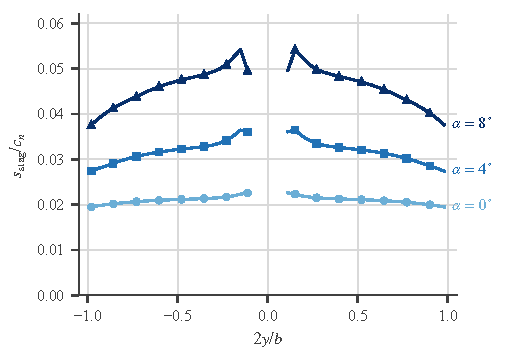
\includegraphics[width=0.85\linewidth]{figures/attachment-offset.pdf}
  \caption{Attachment-line position across the span at $\beta = 0$:
    surface offset of the stagnation point from the leading edge, as a
    fraction of the normal chord, positive onto the lower surface. The
    curves break at the fuselage. The offset is nonzero at $\alpha =
    0$ because the section is cambered.}
  \label{fig:offset}
\end{figure}

Figure~\ref{fig:offset} shows the attachment line at $\beta = 0$.
Every exposed station resolves a stagnation point at every condition,
and the mean offset grows from $0.009\,c_n$ through $0.018\,c_n$ to
$0.027\,c_n$ across the $\alpha$ sweep, tapering toward the tips as
induced downwash relieves the local incidence (the normal-plane
incidence falls from $6.4^\circ$ near the root to $3.3^\circ$ at the
tip at $\alpha = 8^\circ$). The nonzero offset at $\alpha = 0$ is not
noise: a cambered section at zero incidence stagnates below its
leading edge, at $0.009\,c_n$ here --- which is precisely the initial
condition a boundary-layer march loses when it starts from the camber
line's leading edge with $\theta = 0$, the approximation
Section~\ref{sec:wing} exists to remove. Lift coefficients for the
coupled airframe are 0.327, 0.663 and 0.992 across the sweep.

\subsection{Sideslip and the root junction}

\begin{figure}[tb]
  \centering
  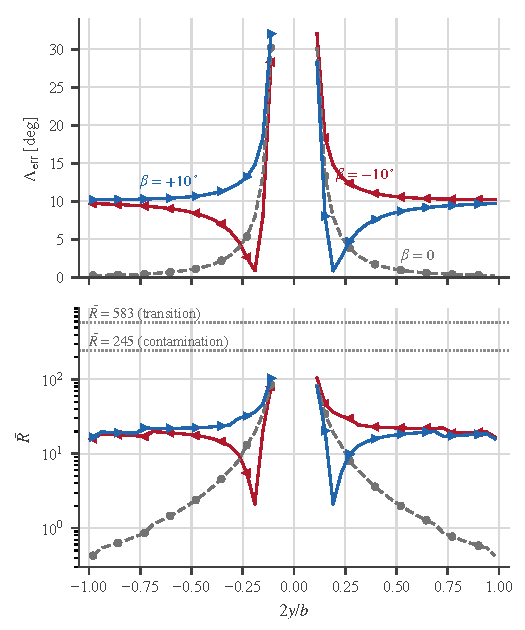
\includegraphics[width=0.9\linewidth]{figures/sideslip-asymmetry.pdf}
  \caption{Effective sweep (top) and attachment-line Reynolds number
    (bottom, log scale) across the span at $\alpha = 8^\circ$, for
    $\beta = -10, 0, +10^\circ$. Positive sideslip blows toward $+y$,
    so the left semi-span ($2y/b < 0$) is windward at $\beta =
    +10^\circ$. Both thresholds of Section~\ref{sec:wing} are shown;
    the whole airframe stays below them.}
  \label{fig:sideslip}
\end{figure}

Figure~\ref{fig:sideslip} contains the two results of this section.
The first concerns the outboard wing. Infinite-swept-wing reasoning
--- and the isolated-wing control case of
Section~\ref{sec:verification} --- says an unswept wing at sideslip is
left/right symmetric, with $\Lambda_{\text{eff}} = |\beta|$ on both
sides. The coupled airframe disagrees: at $\beta = +10^\circ$ the
outboard plateau reads $10.3^\circ$ on the windward wing against
$9.4^\circ$ on the leeward at $\alpha = 8^\circ$, and the split
shrinks with lift ($10.1$ against $9.6$ at $4^\circ$, $9.9$ against
$9.7$ at $0^\circ$) while reversing exactly under $\beta \to -\beta$.
On a planform with identically zero sweep, that asymmetry is supplied
entirely by the induced field --- the trailing-vortex system and the
body's sidewash, neither of which an isolated-section treatment sees.

The second result is the root junction. At $\beta = 0$ the effective
sweep climbs from under $1^\circ$ over the outer wing to $30^\circ$ at
the station beside the fuselage, and $\Rbar$ climbs with it, from
below 2 to 63 at $\alpha = 8^\circ$: the body's crossflow at incidence
must pass around the wing root, and the spanwise flow it acquires in
doing so is what a swept leading edge would otherwise have to supply.
The attachment-line boundary layer of an unswept wing--body junction
is, in this specific sense, all junction and no wing. Sideslip then
splits the junction: the windward root sharpens to $32^\circ$ and
$\Rbar = 66$, while one station out on the leeward side the
spanwise flow passes through a null ($\Lambda_{\text{eff}} =
0.9^\circ$, $\Rbar < 2$) where the body's sidewash cancels the
sideslip component, before recovering to the outboard plateau. Since
leading-edge contamination is seeded at exactly this junction --- it
is Poll's root disturbance~\cite{poll1979} --- the coupled solve's
verdict is that the two roots are not equally exposed --- and its
engineering summary for this airframe is unambiguous: the worst
$\Rbar$ anywhere in the attitude matrix is 135, a factor 1.8 below
the contamination threshold, so the attachment line stays laminar
with margin at every station and attitude examined.

The junction numbers carry a stated modelling sensitivity. Repeating
the sweep with the carry-through vortex enabled moves the outboard
stations almost nowhere --- offsets by less than $0.002\,c_n$ --- but
moves the two stations flanking the fuselage by up to $13^\circ$ of
effective sweep and by up to the full magnitude of their
$\Rbar$. The root spike and its sideslip
split are robust; their third significant figure is not, and the
figures should be read accordingly. A practical meshing note belongs
with this: the trimmed wing's inner trailing legs run along the body
flank at exactly the trim radius, and an azimuthal body refinement
that walks flank control points onto that line degrades the system's
pivot ratio by a factor of five and inflates the solution. The sector
count here (16) keeps them $9.6$~mm clear; the criterion, as always
with a lattice, is distance between singularities and control points,
not panel count.

\subsection{Fuselage stagnation point across the sweep}

\begin{figure}[tb]
  \centering
  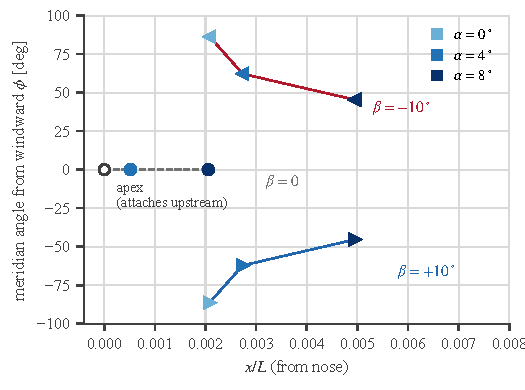
\includegraphics[width=0.85\linewidth]{figures/body-topology.pdf}
  \caption{The fuselage attachment node across the sweep, in axial
    position and meridian angle measured from the windward symmetry
    plane. Marker shade encodes $\alpha$; the $\alpha = \beta = 0$
    case attaches upstream of the first panel ring and is shown open
    at the apex.}
  \label{fig:bodytopo}
\end{figure}

Figure~\ref{fig:bodytopo} tracks the body's primary attachment node.
At $\alpha = \beta = 0$ the flow is axisymmetric and the stagnation
point is the apex itself, upstream of every surface sample --- the
case Section~\ref{sec:body} declines to invent a node for. Every
other condition resolves an interior node, and its migration is the
body-side picture of what the attitude sweep does: pure $\alpha$
walks it aft along the windward meridian ($x/L = 0.0006$ to $0.0021$
from $4^\circ$ to $8^\circ$); adding sideslip rotates it off the
symmetry plane to $86^\circ$, $62^\circ$ and $45^\circ$ from windward
as $\alpha$ grows against a fixed $\beta = 10^\circ$, the node
sliding around the blunt nose toward the resultant of the two
incidences while also moving aft ($x/L = 0.0049$ at the steepest
condition). Reversing $\beta$ mirrors every position exactly. This
node is the seed of every boundary-layer march on the body, and its
strain rate --- evaluated in the local orthonormal frame of
Section~\ref{sec:body}, not from the chart components --- sets
$\theta_0$ there just as the section strain rate does on the wing.

\subsection{Where the flow separates}
\label{sec:separation-results}

\begin{figure}[tb]
  \centering
  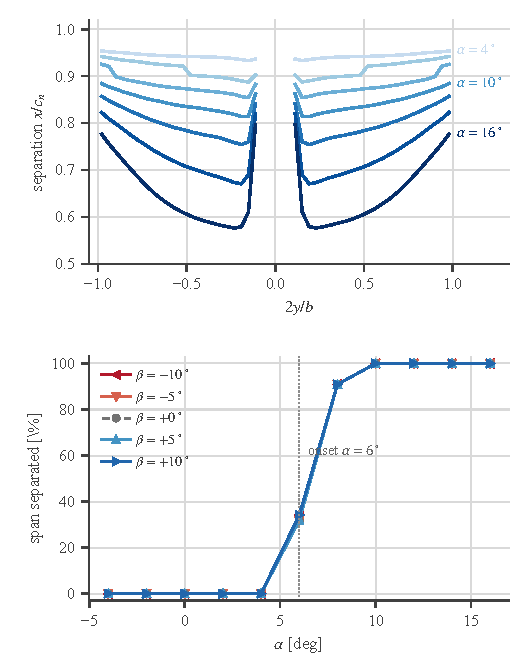
\includegraphics[width=0.85\linewidth]{figures/separation-boundary.pdf}
  \caption{Upper-surface separation from the march of
    Section~\ref{sec:separation}. Top: separation station across the span
    at $\beta = 0$ for increasing incidence;
    separation is most advanced just outboard of the wing root and
    recovers toward the tips. Bottom: fraction of the span separated
    forward of $x/c_n = 0.90$ against $\alpha$, for all five sideslip
    angles --- the curves \emph{collapse} --- on this unswept planform
    the separation boundary is insensitive to sideslip.}
  \label{fig:separation}
\end{figure}

\begin{table}[tb]
  \centering
  \caption{The separation boundary: forwardmost upper-surface
    separation, with the percentage of span separated forward of
    $x/c_n = 0.90$ in parentheses. A dash means no
    station separates forward of that limit.}
  \label{tab:separation}
  \begin{tabular}{rrrrrr}
  \hline
  $\alpha$ & $\beta=-10^\circ$ & $\beta=-5^\circ$ & $\beta=0^\circ$ & $\beta=5^\circ$ & $\beta=10^\circ$ \\
  \hline
     -4 & --- & --- & --- & --- & --- \\
     -2 & --- & --- & --- & --- & --- \\
      0 & --- & --- & --- & --- & --- \\
      2 & --- & --- & --- & --- & --- \\
      4 & --- & --- & --- & --- & --- \\
      6 & 0.88 (34\%) & 0.88 (32\%) & 0.89 (32\%) & 0.88 (32\%) & 0.88 (34\%) \\
      8 & 0.85 (91\%) & 0.85 (91\%) & 0.85 (91\%) & 0.85 (91\%) & 0.85 (91\%) \\
     10 & 0.80 (100\%) & 0.81 (100\%) & 0.81 (100\%) & 0.81 (100\%) & 0.80 (100\%) \\
     12 & 0.74 (100\%) & 0.75 (100\%) & 0.75 (100\%) & 0.75 (100\%) & 0.74 (100\%) \\
     14 & 0.66 (100\%) & 0.66 (100\%) & 0.67 (100\%) & 0.66 (100\%) & 0.66 (100\%) \\
     16 & 0.57 (100\%) & 0.57 (100\%) & 0.58 (100\%) & 0.57 (100\%) & 0.57 (100\%) \\
  \hline
\end{tabular}

\end{table}

The march of Section~\ref{sec:separation} is run at every attitude, and
Fig.~\ref{fig:separation} and Table~\ref{tab:separation} report it. Below
$\alpha = 10^\circ$ the turbulent layer holds close to the trailing edge
at every station: separation exists, as it always does, but sits aft of
$x/c_n = 0.90$ where it is a trailing-edge detail rather than a limit.
At $\alpha = 12^\circ$ it moves forward of $x/c_n = 0.90$ over half the
span (55\%), at $14^\circ$ over 82\%, and by $16^\circ$ it covers
essentially the whole span with the forwardmost station at $x/c_n
\approx 0.80$. The boundary this draws is $\alpha \approx 12^\circ$, and
it is the same at every sideslip angle tested.

The spanwise pattern is worth reading rather than summarizing. Separation
is consistently most advanced just \emph{outboard of the wing root}, near
$2y/b \approx 0.2$, and recovers monotonically toward the tips --- at
$\alpha = 16^\circ$, from $x/c_n \approx 0.80$ inboard to $0.88$ at the
tip. That ordering follows from the same induced field that flattens the
attachment line's offset outboard: downwash relieves the local incidence
toward the tips, so the outer sections run a milder pressure recovery than
the inner ones and hold their layers longer. The practical reading is that
this planform sheds its root first, which is the benign direction --- the
ailerons stay in attached flow past the attitude at which the inboard wing
has let go.

That insensitivity is worth stating explicitly, because it is the
opposite of what the attachment line does. Sideslip moves the attachment
line and its Reynolds number substantially and asymmetrically
(Fig.~\ref{fig:sideslip}), yet leaves the separation boundary alone. The
two are not in conflict: the attachment line responds to the
\emph{spanwise} component of the flow, which is exactly what sideslip
changes, while separation is driven by the chordwise pressure recovery in
the leading-edge-normal plane, which $\beta$ leaves nearly untouched on an
unswept wing. A method that reported the attachment line alone would
suggest a strong sideslip sensitivity that the separation behaviour does
not share, and vice versa. Both are needed to say which one an attitude
limit should be drawn from --- here, separation.

Transition is by laminar separation --- a bubble --- rather than by
Michel's criterion at 2386 of the 2420 station-attitudes in the matrix
(98.6\%; the 34 exceptions cluster at $\alpha = 8$--$12^\circ$). That is
the expected behaviour at $Re_n \approx 3\times10^5$, and it is the
reason the verdict is drawn from turbulent separation rather than from
$\lambda = -0.09$ (Section~\ref{sec:separation}). The caveat stated
there applies to the whole of this subsection: bursting is not modelled,
so $\alpha \approx 12^\circ$ is an upper bound on the attitude at which
the potential-flow coefficients can be trusted, not a predicted stall.

\subsection{Coefficients and stability derivatives}
\label{sec:coefficients}

\begin{table}[tb]
  \centering
  \caption{Force and moment coefficients over the attached portion of the
    attitude matrix. Rows at $\alpha \geq 12^\circ$ are omitted: the
    separation march of Section~\ref{sec:separation-results} places
    separation forward of $x/c_n = 0.90$ there, and a potential-flow
    coefficient past that point is an extrapolation rather than a
    prediction. $C_{D_i}$ comes from a near-field integration and carries a
    spurious body contribution --- it is negative at zero lift and is
    discussed, rather than relied on, in the text. The aerodynamics
    \emph{beyond} this table's edge --- the post-separation coefficients
    toward the flat-plate limit --- is the subject of Part~II.}
  \label{tab:coefficients}
  \begin{tabular}{rrrrrrrrr}
  \hline
  $\alpha$ & $\beta$ & $C_L$ & $C_{D_i}$(near) & $C_{D_i}$(far) & $C_Y$ & $C_m$ & $C_l$ & $C_n$ \\
  \hline
     -4 &     0 & -0.0135 & -0.00617 & 0.00007 & 0.00000 & -0.0097 & 0.00000 & 0.00000 \\
     -4 &    10 & -0.0140 & -0.00448 & 0.00009 & 0.00128 & -0.0087 & -0.00056 & -0.00467 \\
     -2 &     0 & 0.1573 & -0.00420 & 0.00123 & 0.00000 & -0.0138 & 0.00000 & 0.00000 \\
     -2 &    10 & 0.1515 & -0.00263 & 0.00122 & 0.00092 & -0.0127 & -0.00050 & -0.00468 \\
      0 &     0 & 0.3273 & -0.00035 & 0.00488 & 0.00000 & -0.0182 & 0.00000 & 0.00000 \\
      0 &    10 & 0.3164 & 0.00100 & 0.00475 & 0.00025 & -0.0169 & -0.00045 & -0.00469 \\
      2 &     0 & 0.4961 & 0.00530 & 0.01098 & 0.00000 & -0.0228 & 0.00000 & 0.00000 \\
      2 &    10 & 0.4801 & 0.00635 & 0.01067 & -0.00073 & -0.0214 & -0.00039 & -0.00470 \\
      4 &     0 & 0.6635 & 0.01265 & 0.01952 & 0.00000 & -0.0277 & 0.00000 & 0.00000 \\
      4 &    10 & 0.6423 & 0.01333 & 0.01895 & -0.00199 & -0.0261 & -0.00034 & -0.00469 \\
      6 &     0 & 0.8289 & 0.02159 & 0.03044 & -0.00000 & -0.0327 & 0.00000 & 0.00000 \\
      6 &    10 & 0.8027 & 0.02182 & 0.02955 & -0.00352 & -0.0310 & -0.00028 & -0.00468 \\
      8 &     0 & 0.9920 & 0.03198 & 0.04370 & 0.00000 & -0.0380 & 0.00000 & 0.00000 \\
      8 &    10 & 0.9608 & 0.03170 & 0.04241 & -0.00530 & -0.0361 & -0.00023 & -0.00467 \\
     10 &     0 & 1.1525 & 0.04368 & 0.05924 & 0.00000 & -0.0434 & 0.00000 & 0.00000 \\
     10 &    10 & 1.1164 & 0.04282 & 0.05747 & -0.00729 & -0.0414 & -0.00017 & -0.00465 \\
  \hline
\end{tabular}

\end{table}

\begin{table}[tb]
  \centering
  \caption{Stability derivatives at $\beta = 0$ over the attached
    attitudes, computed by central differences on the coupled
    wing--body--duct system. Angle derivatives are per radian; rate
    derivatives are per unit reduced rate ($q\bar{c}/2V$, $pb/2V$,
    $rb/2V$).}
  \label{tab:derivatives}
  \begin{tabular}{rrrrrrrrr}
  \hline
  $\alpha$ & $C_{L_\alpha}$ & $C_{m_\alpha}$ & $C_{Y_\beta}$ & $C_{l_\beta}$ & $C_{n_\beta}$ & $C_{m_q}$ & $C_{l_p}$ & $C_{n_r}$ \\
  \hline
     -4 & 4.899 & -0.113 & 0.0090 & -0.0032 & -0.0273 & -0.190 & -0.4579 & 0.0008 \\
     -2 & 4.883 & -0.121 & 0.0068 & -0.0029 & -0.0274 & -0.193 & -0.4586 & 0.0011 \\
      0 & 4.856 & -0.129 & 0.0028 & -0.0026 & -0.0274 & -0.197 & -0.4588 & 0.0014 \\
      2 & 4.817 & -0.136 & -0.0030 & -0.0023 & -0.0275 & -0.200 & -0.4584 & 0.0017 \\
      4 & 4.767 & -0.142 & -0.0106 & -0.0020 & -0.0274 & -0.202 & -0.4574 & 0.0020 \\
  \hline
\end{tabular}

\end{table}

Tables~\ref{tab:coefficients} and~\ref{tab:derivatives} are the practical
output of the whole exercise: a coefficient and derivative set over the
attitude matrix, restricted to the attitudes at which
Section~\ref{sec:separation-results} says the potential-flow answer is
still meaningful. Restricting them is the point. A panel method will
return a lift coefficient at any incidence it is asked for, and the
returned number at $\alpha = 16^\circ$ ($C_L = 1.62$) is arithmetically
sound and physically meaningless with most of the upper surface
separated. Having the separation march in the same solve is what lets the
table be truncated on evidence instead of on a rule of thumb.

The derivatives are computed on the \emph{coupled} system, not on the wing
alone. That matters most for $C_{n_\beta}$, which is negative across the
whole matrix --- this configuration is directionally unstable, as a
wing--body with no vertical surface must be, since the fuselage's Munk
moment is destabilizing and there is nothing aft to oppose it. A
wing-only derivative calculation would report a value near zero and miss
the conclusion entirely. $C_{m_\alpha}$ is likewise small and negative,
the modest static margin that follows from a moment reference point
slightly ahead of the wing's aerodynamic centre, and it is only correct
because the reference point is carried through the contract-to-solver
frame rotation; skipping that flip places it an equal distance the wrong
side of the origin and inflates $C_{m_\alpha}$ by an order of magnitude
through a spurious moment arm of about one body length.

Roll damping is the derivative worth checking a method against, because
it has a textbook value: $C_{l_p}$ comes out at $-0.458$ at $\alpha = 0$
and drifts only to $-0.440$ by $16^\circ$, against the standard result
near $-0.45$ for an unswept wing of this aspect ratio.

$C_{D_i}$ is reported twice in Table~\ref{tab:coefficients}, and the
reason is worth setting out because the near-field column is unusable on
this configuration in a way that is easy to miss.

Forces are ordinarily integrated in the NEAR field here, by applying
Kutta--Joukowski at each bound-vortex midpoint. On a wing alone that is
sound. On a coupled configuration it is not: the near-field $C_{D_i}$ is
\emph{negative} at $\alpha = -4^\circ$, where the lift is essentially zero
and induced drag must vanish, and fitting the $\beta = 0$ column to
$C_{D_i} = C_{D_i,0} + kC_L^2$ returns $C_{D_i,0} = -0.0037$ with a $k$
implying a span efficiency of 1.53 --- not merely optimistic but
impossible, since $e \leq 1$ for any planar wing.

The cause is worth stating precisely, because the tempting explanation is
wrong. It is \emph{not} that the discretized body carries a spurious
force: closed bodies in this solver satisfy d'Alembert to machine
precision in uniform flow, $|F|/(q A) \sim 10^{-16}$, and the force the
body carries in the coupled solve is physical --- it sits in the wing's
upwash and accounts for about 8\% of the configuration's lift. The cause
is that near-field induced drag is a small difference of much larger
quantities. It is the streamwise component of forces dominated by lift, so
its relative error is amplified by the lift-to-drag ratio and converges
slowly for that reason alone. Introducing a body substantially alters the
induced velocity at the wing's bound vortices, most of all near the root,
and adds a pressure integration over the body in a strongly non-uniform
field. Both errors are negligible beside lift --- which is why $C_L$ and
the moments are unaffected, consistent with the lift-slope and
roll-damping checks above --- and comparable with induced drag, which is a
far smaller number.

The far-field column removes both symptoms, and it is worth setting out
why it is \emph{structurally} immune rather than merely better conditioned.

Take a control volume closed by a plane far downstream --- the Trefftz
plane --- and let $\phi$ be the perturbation potential in it. All the
disturbance the configuration leaves behind is the wake's crossflow
kinetic energy, so the induced drag is
%
\begin{equation}
  \label{eq:energy}
  D_i = \frac{\rho}{2}\iint_{T}\left|\nabla_{\!2}\phi\right|^2
        \mathrm{d}y\,\mathrm{d}z ,
\end{equation}
%
with $\nabla_{\!2}$ the in-plane gradient. Far downstream the streamwise
perturbation has decayed and $\phi$ satisfies the two-dimensional Laplace
equation in the plane, so Green's first identity converts
Eq.~\eqnref{eq:energy} into a contour integral around the wake trace $C$,
%
\begin{equation}
  \label{eq:green}
  D_i = -\frac{\rho}{2}\oint_{C}\Delta\phi\,
        \frac{\partial\phi}{\partial n}\,\mathrm{d}\ell ,
\end{equation}
%
the outer boundary contributing nothing because $\phi$ decays like a
two-dimensional doublet. On a lifting surface's wake the potential jump is
the bound circulation, $\Delta\phi = \Gamma(y)$, and the normal derivative
is the downwash, giving
%
\begin{equation}
  \label{eq:trefftz}
  D_i = -\frac{\rho}{2}\int_{-b/2}^{b/2}\Gamma(y)\,w_T(y)\,\mathrm{d}y .
\end{equation}
%
The factor of one half in Eq.~\eqnref{eq:trefftz} is often mistaken for a
convention. It is not. $w_T$ is the downwash induced \emph{in the Trefftz
plane}, where each trailing filament runs from $-\infty$ to $+\infty$ and
acts as a full two-dimensional vortex; at the lifting line the same
filament is semi-infinite and induces half as much. Substituting the
lifting-line downwash into Eq.~\eqnref{eq:trefftz} therefore halves the
drag while leaving every trend intact --- an error that survives a sign
check and a convergence study alike.

The structural point follows from Eq.~\eqnref{eq:green} directly. A closed
non-lifting body carries a source distribution, not a vortex sheet. Its
potential is single-valued, so $\Delta\phi = 0$ on any trace it leaves,
and it contributes nothing to the contour integral \emph{regardless of how
it is discretized}. That is why the far-field result cannot inherit the
near-field evaluation's error: the body is not merely small in
Eq.~\eqnref{eq:green}, it is absent from it.

Two approximations remain and should be named. The plane is taken normal
to the $x$ axis rather than to the freestream, which is consistent with
this solver's frozen wake --- the vorticity the plane is meant to
intercept runs along $x$ --- and carries the same $O(\alpha^2)$ error the
frozen wake already does. And Eq.~\eqnref{eq:trefftz} presumes the sheet
reaches the plane without rolling up. Roll-up redistributes $\Gamma(y)$
but conserves the impulse that sets $D_i$, so the leading-order result is
unaffected~\cite{katzPlotkin2001}.

With this in place the zero-lift intercept falls from $-0.0037$ to
$-0.0003$, and $C_{D_i}$ is positive at every attitude in the matrix.

Span efficiency then requires one care in its formation, which is worth
stating because getting it wrong looks exactly like a defect in the
integral. The far-field drag belongs to the \emph{lifting system}, since
only the lifting system sheds a wake, so it must be compared against the
lifting system's lift. On this airframe the fuselage carries about 9\% of
the total, and using the configuration $C_L$ returns $e = 1.17$ --- still
above the bound --- while the wing's own lift returns $e = 0.965$, with
per-condition values between 0.96 and 0.99 across the attached range. That
is the physically admissible answer, and it is the one the method was
always producing; only the comparison was mismatched.

$C_{m_q}$ deserves a caveat rather than a comparison. It is reported as
roughly $-0.20$, and that value is a floor rather than an estimate. The
lattice carries one chordwise row per strip, so every bound vortex lies on
the quarter-chord line and every control point a half chord behind it: a
pitch rate about a point \emph{on} that line adds the same upwash at every
control point, a uniform change in effective incidence that moves $C_L$
but exerts no moment about the line it acts on. Pitch damping here
therefore arises entirely from the offset between the moment reference
point and the quarter-chord line, and the chordwise redistribution of load
that supplies most of a real wing's $C_{m_q}$ is absent by construction.
Reporting the number with that limitation attached is more useful than
either omitting it or presenting it as converged; a chordwise-resolved
lattice would be required to do better, at a cost the rest of this method
does not otherwise incur.

\subsection{The skin-flow portrait}

\begin{figure}[tb]
  \centering
  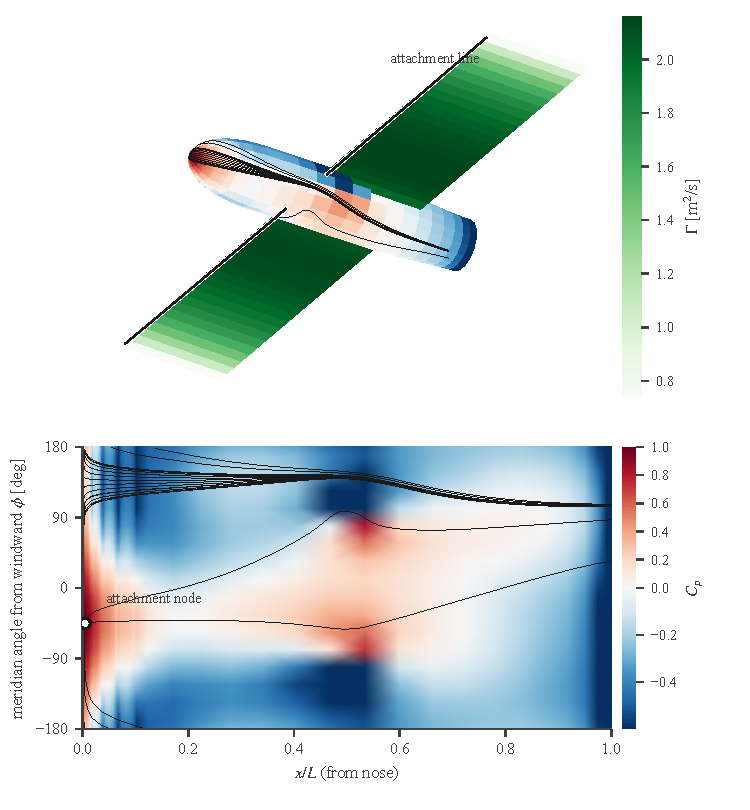
\includegraphics[width=\linewidth]{figures/body-streamlines.pdf}
  \caption{The airframe at $\alpha = 8^\circ$, $\beta = +10^\circ$:
    orthographic view from the windward-left quarter (top) and the
    unwrapped fuselage meridian map (bottom). The fuselage carries its
    surface streamlines colored by $C_p$ referenced to the
    translational freestream; the wing lattice is colored by its
    solved bound circulation, with the computed attachment line drawn
    on the lower surface it lies on. Body streamlines emanate from the
    attachment node on the windward-left flank and converge into a
    single leeward line; the duct-exit base annulus is the open
    downstream boundary.}
  \label{fig:portrait}
\end{figure}

Figure~\ref{fig:portrait} assembles the whole airframe at the
steepest combined condition, $\alpha = 8^\circ$ with $\beta =
+10^\circ$. On the wing, the spanwise circulation distribution and
the attachment line are shown together, which is the pairing this
method exists to produce: the lattice supplies the loading and the
local flow, and the section solve turns that local flow into the line
the boundary layer starts from, drawn here in the three-dimensional
positions the analysis reports, running just below each leading edge
from root to tip. On the body, the distinguished streamlines of the attachment node fan
out of the windward-left flank of the nose, wrap the body, and
collect into a single bundle on the leeward side --- rotated well off
the geometric top of the body, as the combined incidence demands. The
convergence of that bundle is the signature the spreading metric $h$
of Section~\ref{sec:body} exists to carry: streamlines crowding
together is precisely $h$ collapsing, which is what an integral
method needs to know approaching separation. What the inviscid field
does \emph{not} contain is an interior separation critical point ---
the surface flow leaves the patch through the base annulus, which on
this airframe is a duct exit rather than a closed tail, and no zero
of the tangential velocity exists forward of it at any condition
examined. That is the honest division of labor: an attached potential
flow has no business declaring separation, and the topology hands the
boundary layer everything it needs --- the node to start from, the
streamlines to march along, $U_e(s)$ and $h(s)$ down each one --- to
declare it itself.

\section{Conclusions}

A coupled wing--body panel method can supply everything an integral
boundary-layer method needs to begin --- attachment location, edge
velocity distribution, initial momentum thickness, and streamline
spreading --- provided the wing and the body are treated according to what
they actually are. The body's stagnation points are found by searching a
real surface field; the wing's cannot be, and must come from a
two-dimensional solve of the reconstructed thick section driven by the
lattice's induced flow.

Spending those initial conditions on a march to separation turns the
method into something a configuration study can use directly: a
coefficient and derivative table over an attitude matrix, bounded by
evidence rather than by convention. A panel method returns a lift
coefficient at any incidence it is asked for, and the burden of knowing
which of those numbers to believe has conventionally fallen outside the
method. Carrying the boundary layer's starting state through to a
separation criterion moves that judgement inside it.

Three formulation choices proved to be load-bearing rather than
discretionary. Surface strain rates must be differenced from the
tangential velocity in a local orthonormal frame, not from contravariant
components whose chart factors do not converge away. The wing's section
problem must be posed in the plane normal to the leading edge, not
streamwise, because only the former represents the asymmetry that sideslip
imposes on a swept wing's attachment line --- an asymmetry that determines
which wing is closer to leading-edge contamination, and therefore cannot
be treated as a second-order correction. And Thwaites' integral must be
evaluated exactly on the first step out of the attachment point, where the
trapezoid rule is wrong by a factor of three and $\theta_0$ by $\sqrt{3}$
--- an error invisible to a march that starts at a leading edge with
$\theta = 0$, and therefore one that only appears once the attachment
point is located properly.

The results also separate two sensitivities that are easily conflated.
Sideslip moves the attachment line strongly and asymmetrically while
leaving the separation boundary essentially unchanged, because the two
respond to different components of the same flow: the attachment line to
the spanwise component, separation to the chordwise pressure recovery.
Neither quantity alone would have revealed that, and a configuration limit
drawn from the wrong one would be wrong in a way that looks reasonable.

Everything here ends at the separation boundary, deliberately: the
coefficient tables stop where the march says the potential-flow answer
stops being a prediction. Part~II of this series takes up what lies
beyond --- the post-separation coefficients, anchored on the computed
separation points and on the classical flat-plate limits, out to
$90^\circ$ of incidence.

\section*{Acknowledgments}

This work was supported by the Istanbul Technical University Scientific
Research Projects Coordination Unit (\.IT\"U BAP) under project
MGA-2026-48282, ``JETTAIL: Design, Control, and Autonomous Mission
Capability Development of a Jet-Flow-Vectored EDF-Based Tail-Sitter VTOL
UAV.'' The airframe used as the application case in
Section~\ref{sec:application} is the demonstrator of that project.

% TODO: any further funding/collaborators. AI-assistance disclosure per
% AIAA policy. Verify the English rendering of the project title against
% the award letter (kept identical to the SciTech draft's wording, which
% is the same award).

\bibliographystyle{aiaa}
\bibliography{references}

\end{document}
